\chapter{提案手法}

\section{概要}
本章では,本研究で提案するシステムについて説明する.
本研究では,識別精度を犠牲にすることなくアノテーションコストを抑える病理画像解析のための深層能動学習システムを構築する.
高精度を達成するために識別器にConvolutional Neural Networkを採用し,少ないラベル数でも学習を収束させるために
ImageNetで学習済みのpretrained-networkの重みをもとにfine-tuningによって学習を行う.
一般画像認識のために学習されたモデルでも,医療画像解析への転移学習は幅広いタスクに対して有効であると知られているため,妥当だと考えられる.

また,前章で述べた深層学習と能動学習の組み合わせの問題に対する解決するためのアプローチとして,Query-By-Dropout-Predictionsを提案する.
不確かさを定義しない多層ニューラルネットワークのパラメータを更新するサンプルを効率的に見つけるために,
正則化に使用されるDropoutを利用して擬似的にQuery-By-Committeeを再現する.
さらに,医療画像解析において重要であると考えられる,様々な変形への不変性の担保を考慮し,
各Committeeのprediction時にもランダムなData Augmentationを利用することで,
識別に有効なサンプルのみではなく不変性を確保するために有効であるサンプルをクエリとして選択することを考える.
また,WSIにおける大量の画像パッチを能動学習の枠組みで扱うための実用的な方法を提案する.
さらに,能動学習において一般に問題となるサンプリングバイアスやバッチ能動学習におけるクエリ内の情報重複問題を解決するためにクラスタリング手法を採用し,
その際に用いる特徴量について妥当だと考えられるものを実験から選定した.

以下の節では,それぞれについて詳細を説明する.

\clearpage

\begin{figure}[tbp]
    \label{fig:overview}
     \begin{center}
      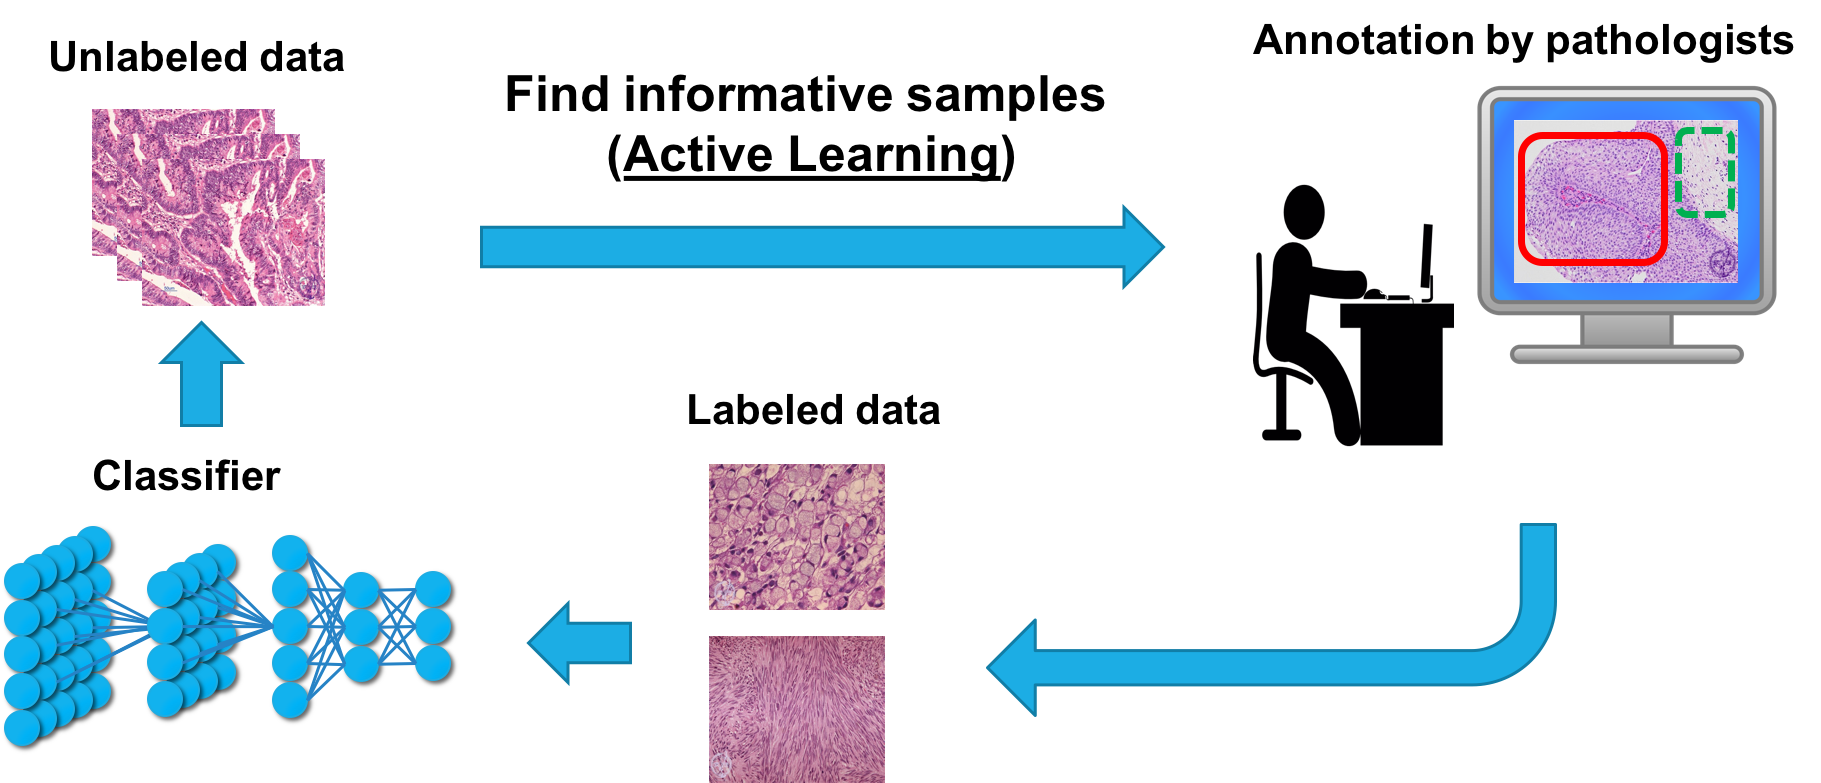
\includegraphics[width=120mm]{figures/overview.png}
     \end{center}
    \caption{本研究で提案するシステムの概念図}
\end{figure}

\section{Query by Dropout Predictions}
多層ニューラルネットワークによって識別問題を解く際には,最終出力が各ラベルに対応する確率分布となるように設計して学習を行う.
多層ニューラルネットワークを能動学習に利用する際にはこの確率分布のエントロピーの大きさなどを利用して不確かさを定量評価し,
Uncertainty Samplingによってクエリ選択を行う.
しかし,前章で述べたように,ニューラルネットワーク自体のパラメータに対する不確かさをモデリングしているわけではない.
このように不確かさを陽にモデル化しない識別器を利用した能動学習においては,
バージョン空間を近似的に保持することで有効なサンプルを選択するQuery By Committeeを用いる事が多いが,
多層ニューラルネットワークのように非常に計算コストの重いモデルを複数同時に保持し学習を行うことはメモリ,
計算時間等様々な問題で現実的ではないという問題があった.
そこで,本研究では,多くの深層学習のアーキテクチャにおいて,正則化のために利用されるDropoutによって,
本体のネットワークからサンプリングされた部分ネットワークをCommitteeとみなし,
それらの予測の不一致度を利用して近似的にQuery-By-Committeeを行う手法を提案する(Fig.\ref{fig:query_by_dropout}).
つまり,本体のネットワーク$\mathcal{M}$から生成された部分ネットワーク$\mathcal{C} = \{\mathcal{M}_{p_1}, \mathcal{M}_{p_2}, \dots, \mathcal{M}_{p_c} \}$を用いて
以下のKullback–Leiblerを計算する.
\begin{eqnarray}
    score(x) =  -  \frac{1}{C} \sum_{c=i}^C KL \, (P_{\theta^{(c)}} || P_C)
\end{eqnarray}
これらの部分ネットワークがCommitteeとして利用されるためには,それらが訓練データに対してはConsistentであり,
かつ,それぞれの未知データに対する出力には分散を持つ必要がある.
この性質について実験で検証し,Uncertainty Samplingのみを利用する方法と比較する.

\begin{figure}[tbp]
     \begin{center}
      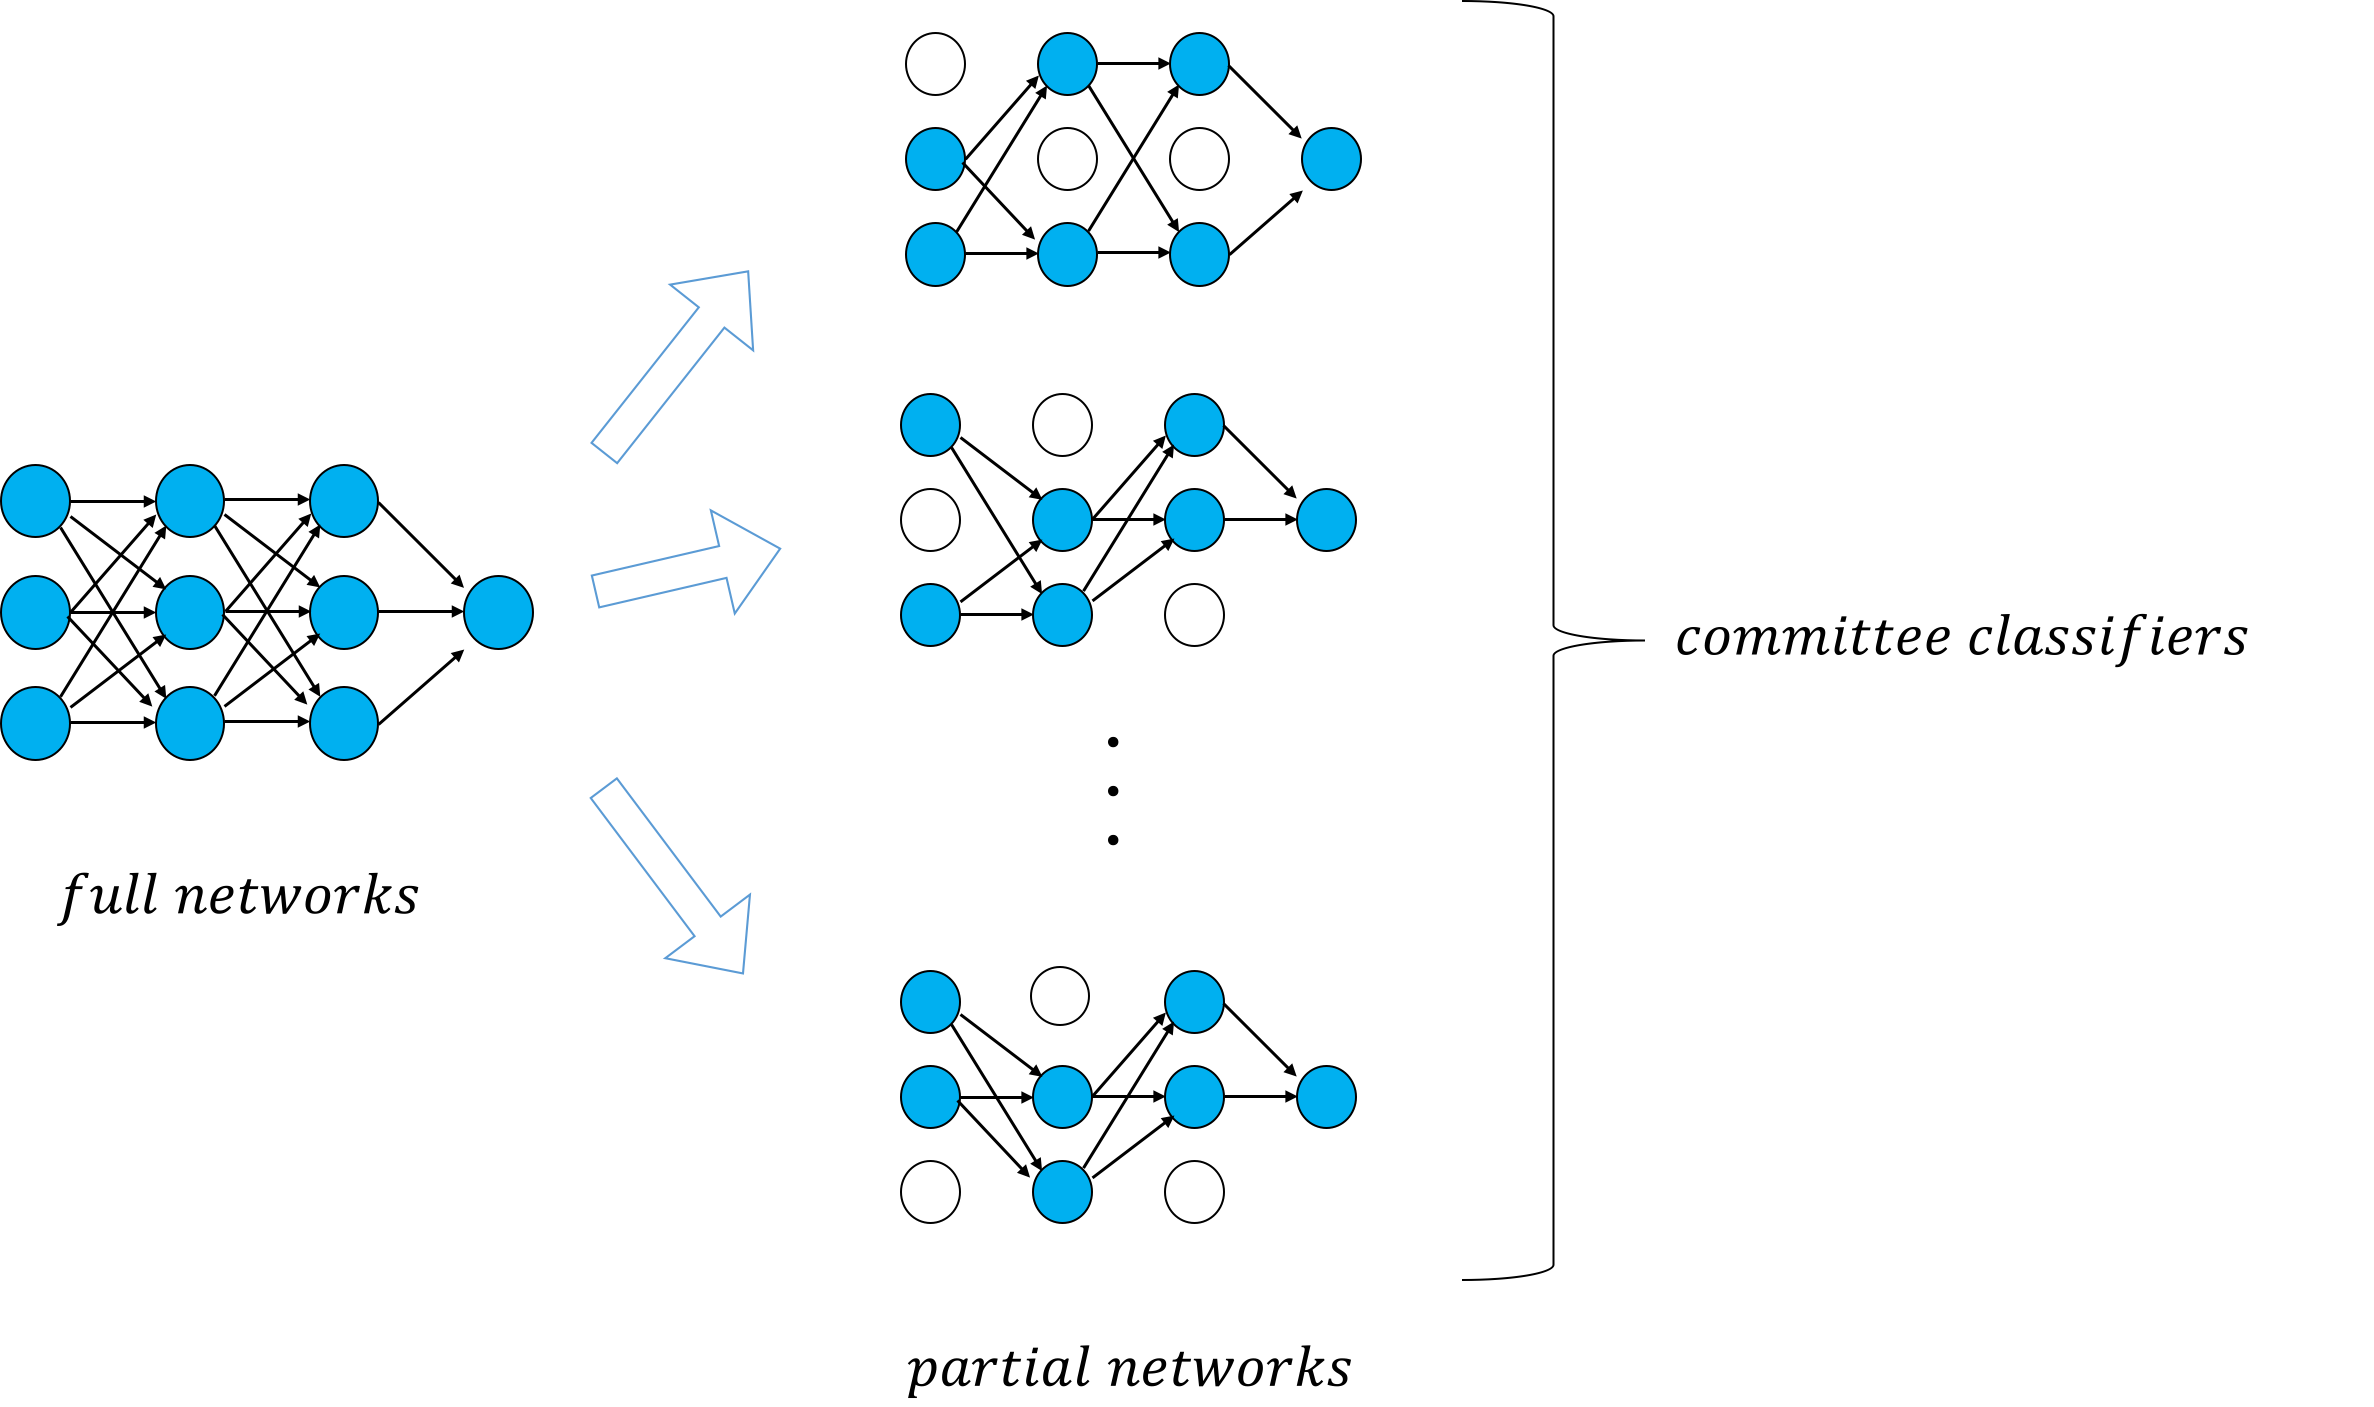
\includegraphics[width=120mm]{figures/query_by_dropout.png}
     \end{center}
    \caption{\label{fig:query_by_dropout}提案するQuery-By-Dropout-Predictionsの概要図.Dropoutによってサンプリングされた部分ネットワークによってCommitteeを形成する.}
\end{figure}

\section{推論時でのData Augmentationの利用}
CNNを学習させる際,訓練時に画像に対してData Augmentationを利用することで不変性を獲得させ,結果的に汎化性能を向上させる工夫が用いられる.
ラベル付きデータが少ない場合は特に過学習を防ぐために有効であると知られており,本研究でも識別器の学習に使用する.
第2章で述べたように,医療画像解析では一般画像認識と比較してモデルが獲得すべき不変性が多く存在する.
特に病理画像解析では,向き,回転,位置に対する不変性,色相,輝度に対する不変性を獲得しているのが望ましい.

前節で,Dropoutによって部分ネットワークCommitteeを生成することで不一致度を測る手法を提案したが,
本研究ではそれだけではなく,Data Augmentationを推論時にも利用することで,さらに効率的にモデルを更新するサンプルを選択する手法を提案する.

\section{提案手法の動作原理}
% pre-trained networkを利用する.
通常Dropoutは全結合層のみで使用されることが多い.
すなわち,Dropoutによってサンプリングされた各CommitteeはそれぞれCNNの畳み込み層から抽出された特徴量に対する識別境界面の引き方が異なっていると考えられる.
この時,各Committeeの予測の不一致度が高くなるようなサンプルは識別境界を大きく変更させるために有効であると考えられる.
しかしCNNにおいては,識別境界の決定だけでなく特徴抽出の表現学習も重要な因子である.
そこで,訓練時のみではなく推論時にも各予測を出力するためにData Augmentationを利用することで識別境界の決定でなく
特徴抽出のために有用であるサンプルを取得できるのではないかと考えられる.
提案手法の動作原理のイメージ図を図\ref{fig:how_it_works}に示す


\begin{figure}[tbp]
     \begin{center}
      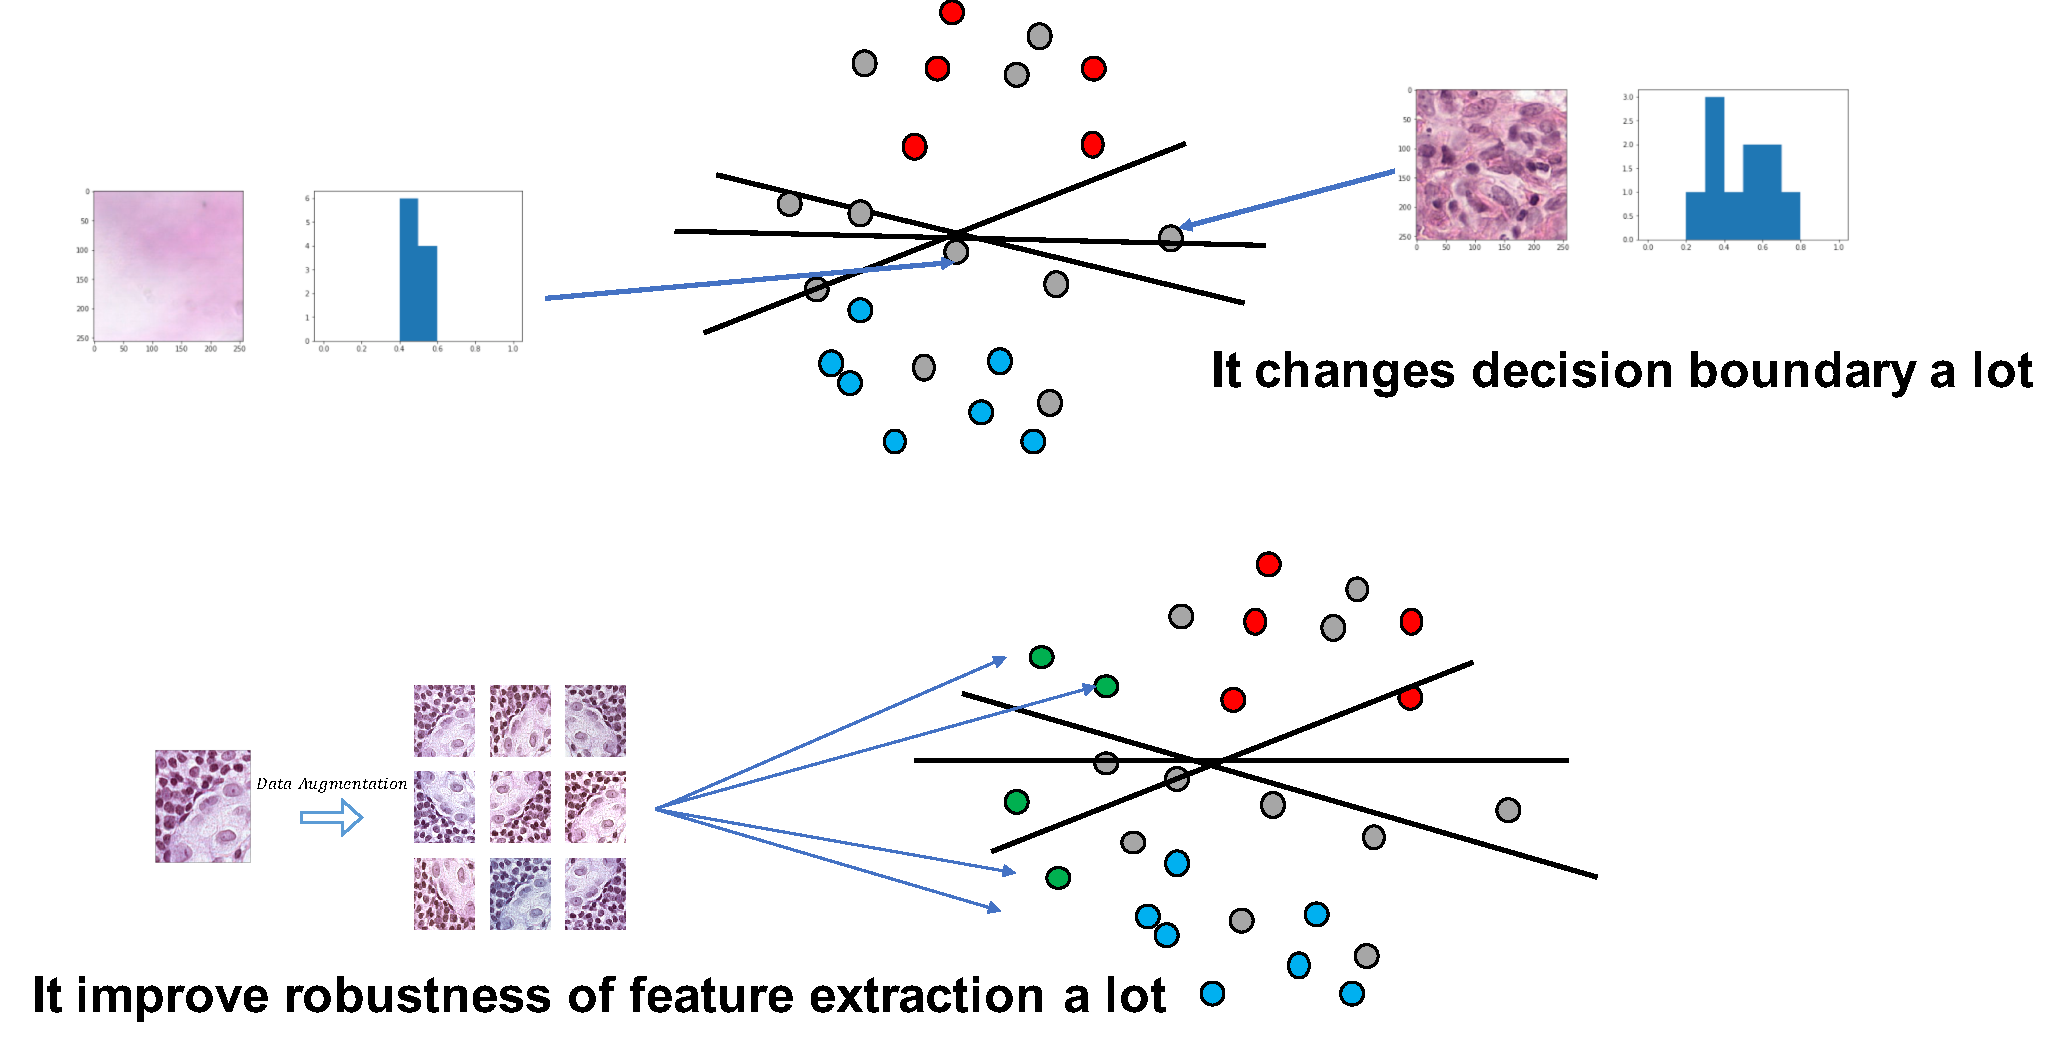
\includegraphics[width=120mm]{figures/how_it_works.pdf}
     \end{center}
    \caption{\label{fig:how_it_works}提案手法の動作原理のイメージ図.Dropoutによる不一致度の定量評価をData Augmentationを併用することで効果を高める.}
\end{figure}


\section{ラベルなしデータプールのサンプリング}
病理画像では,1枚のWSIに数十万枚の画像パッチが含まれるため,訓練時に使用できるWSIから全ての画像パッチを取り出しラベルなしデータセット$\mathcal{U}$として利用した場合,
その数は数百万にのぼってしまう.
このサンプルプールからあるクエリ選考基準を最大化するサンプルを選択するのは計算コストの点から実用上困難である.
しかし予め一定数をサンプリングして固定の$\mathcal{U}$を使用するのは,利用可能なデータ数を制限することになってしまう.
そこで,クエリ問い合わせ毎に利用可能な画像パッチ全体から一部をサンプリングすることで$\mathcal{U}_i$を作成し,
この中からモデル更新に寄与するサンプルを選択することで,現実時間内で最適なクエリを探索可能にしつつ,
利用可能データを最大限に利用する手法を提案する.

\section{バッチ型能動学習への拡張}
能動学習では,クエリ問い合わせを行いラベルデータを拡充するごとに,識別器をfrom scratchで学習させるのが一般的である.
深層学習器を能動学習に利用する場合,一度の再学習に大きな計算コストがかかってしまうため,
各クエリ問い合わせにおいて複数のサンプルにラベルを付与するバッチ型能動学習を採用するのが適当であると考えられる.
一度に投げるクエリ内での情報の重複を避けるために何らかの工夫をする必要があるが,
2章で述べたような劣モジュラ関数を設計するのは深層学習を利用する場合計算コストの観点から難しい.
そこで,本研究では予めラベルなしデータをクラスタリングし,一度のクエリでは同一のクラスターに属するサンプルを2つ以上選択しないことで,情報の重複を避ける.
また,クラスタリングに使用する特徴量の候補として,以下の3つを考慮した.

\subsubsection{Hand-crafted feature}
第2章で述べたように,病理画像解析にはテクスチャ解析で用いられる技術がしばしば使用される.
ここでは,パターンベースの特徴量で,位置不変性と輝度変化への頑健性を有するLocal Binary Pattern (LBP)\cite{ojala2002multiresolution}を採用する.
実際には,回転不変性を担保させるようにLBPを改良したimproved LBPを利用した.

\subsubsection{CNNの中間特徴量}
Imagenetで学習された特徴量は様々なタスクに有用であるとされており,多数の医療画像解析で利用されている.
本研究ではGoogleNet\cite{szegedy2015going}の中間特徴量を空間方向に平均を取ることで圧縮した512次元を利用した.

\subsubsection{compact bilinear poolingによる特徴量}
近年では,深層学習を用いたテクスチャ解析に関する研究も盛んに行われている.
Bilinear Pooling \cite{lin2015bilinear}は,CNNの中間特徴量同士の相関を計算し空間方向に平均を取ることで獲得される自己相関行列を特徴量として利用する手法である.
\begin{eqnarray}
G_{ij} = \sum_k{F_{ik} F_{jk}}
\end{eqnarray}
$G$はBilinear Poolingによって得られる自己相関行列,$F$はCNNの中間特徴マップ,$k$は画像中の位置情報を表す.
一般にCNNの特徴量次元(チャンネル数)は256 〜 512の大きな値であるため,直接計算した場合非常に高次元な値となってしまう.
そこで,ランダム行列によってBilinear Poolingによって得られる特徴量を近似する手法である
Compact Bilinear Pooling(CBP)\cite{gao2016compact}を本研究では採用する.
ランダム行列の次元を増やすほどBilinear Poolingの近似精度が上がるという特徴になっている.
CNNを用いたテクスチャ特徴量として,GoogleNet\cite{szegedy2015going}の中間特徴量をCBPによって512次元まで圧縮したものを採用する.

\section{アルゴリズムの詳細}

本研究で提案するアルゴリズムの詳細を以下に示す(Algorithm\ref{algo:dal}).

\begin{description}
    \item[step1] ラベルなしデータセット$\mathcal{U}$,初期ラベル付きデータセット$\mathcal{L}$を準備する
    \item[step2] CNNモデル$\mathcal{M}$にpretrained modelの重みをセットする
    \item[step3] $\mathcal{L}$を利用して,$\mathcal{M}$をfine-tuningにより学習
    \item[step4] $\mathcal{U}$から$\mathcal{U}_i$をサンプリングする
    \item[step5] K-meansによって$\mathcal{U}_i$を$\mathcal{U}_{i_1}, \mathcal{U}_{i_2}, \dots, \mathcal{U}_{i_k}$にクラスタリングする
    \item[step6] Dropoutにより$\mathcal{L}$からCommittee $\mathcal{C} = \{\mathcal{M}_{p_1}, \mathcal{M}_{p_2}, \dots, \mathcal{M}_{p_c} \}$を生成
    \item[step7] Committee $\mathcal{C}$ を利用し$\mathcal{U}$のdisagreement scoreを計算
    \item[step8] $\mathcal{U}$からスコアが高いものを,同一クラスターからは二つ以上選択しないように選び,クエリ$Q$を作成
    \item[step9] $Q$にラベルを付与し,$\mathcal{L}$に追加する
    \item[step10] モデルのvalidation scoreが望みの値を達成するまでstep3〜step9を繰り返す
\end{description}


\begin{algorithm}[h]
    \caption{Deep Active Learning for Pathological Image Analysis}
    \label{algo:dal}
    \begin{algorithmic}
        \STATE \textbf{Input: } 
        unlabeled dataset $\mathcal{U}$,
        initial labeled datset $\mathcal{L}$,
        clustering size $k$, 
        active sampling size $K$,
    \end{algorithmic}

    \begin{algorithmic}
        \STATE \textbf{Output: } paramters of network $\mathcal{M}$
    \end{algorithmic}
    
    \begin{algorithmic}[1]
        \STATE Initialize pre-trained network $\mathcal{M}_{pretrained}$
        \REPEAT
            \STATE $\mathcal{M} \leftarrow train (\mathcal{M}_{pretrained}, \mathcal{L})$
            \STATE sample partial unlabeled dataset $\mathcal{U}_i$ from $\mathcal{U}$
            \STATE Perform k-means clustering and devide $\mathcal{U}_i$ to disjoint clusters $\mathcal{U}_{i_1}, \mathcal{U}_{i_2}, \dots, \mathcal{U}_{i_k}$
            \STATE sample committees $\mathcal{C} = \{\mathcal{M}_{p_1}, \mathcal{M}_{p_2}, \dots, \mathcal{M}_{p_c} \}$ from $\mathcal{M}$ using $dropout$ 
            \FOR {$each \; x \in \mathcal{U}$}
                \STATE $score (x) \; = disagreement\_score \; (x, \; \mathcal{C}) $
            \ENDFOR
            \STATE $\mathcal{Q} \leftarrow \O$, $\mathcal{D} \leftarrow \O$
            \WHILE{$len(\mathcal{Q}) < K$}
            \STATE $x^{\ast} = \argmax_{x \in \mathcal{U}_i} score(x)$
            \STATE $idx = cluster(x^{\ast})$
            \IF{$idx \notin D$}
            \STATE $\mathcal{Q} \leftarrow \mathcal{Q} \cup \{x^{\ast}\}, \mathcal{D} \leftarrow \mathcal{D} \cup \{idx\}$

            \ENDIF

            \ENDWHILE
            \STATE Query labels for $\mathcal{Q}$
            \STATE $\mathcal{L} \leftarrow \mathcal{L} \cup \mathcal{Q}$

      \UNTIL{perfomance is satisfactory}
    \end{algorithmic}
  \end{algorithm}
  
